\documentclass[final,t]{beamer}
\mode<presentation>{ \usetheme{Major} }
\usepackage{times}
\usepackage{amsmath,amsthm, amssymb, latexsym}
\boldmath
\usepackage[english]{babel}

\usepackage{relsize}
\usepackage{multirow}
\usepackage{qtree}
\usepackage{stmaryrd}
\usepackage{booktabs}

%  \usepackage[font=small,format=plain,labelfont=bf,up,textfont=it,up]{caption}
\usepackage[font=normalsize,labelfont=small,bf,margin=2cm]{caption}
\usepackage[latin1]{inputenc}
\usepackage[orientation=portrait,size=a0,scale=1.4,debug]{beamerposter}
\usepackage{color,listings}
\usepackage{calc,xcolor}
\usepackage[absolute,overlay]{textpos}
\usepackage{smartdiagram}

\usepackage{wrapfig}

\definecolor{lightblue}{rgb}{.85,.85,1} % 217 217 255
\definecolor{lightorange}{rgb}{1,.8,.6} % 255 204 153
\definecolor{lightgreen}{rgb}{.77,.91,.5} % 196 232 128
\definecolor{lightyellow}{rgb}{1,.98,.6} % 255 250 153


\newsavebox\CBox
\newenvironment{ColorBox}[3][black]{
    \par\noindent
    \def\borderColor{#1}\def\bgColor{#2}
    \begin{lrbox}{\CBox}
    \minipage{#3-2\fboxsep-2\fboxrule}
}{
    \endminipage\end{lrbox}%
    \fcolorbox{\borderColor}{\bgColor}{\usebox\CBox}\par
}

\lstset{language=java}
\lstset{breaklines=true}
\lstset{showstringspaces=false}
\lstset{tabsize=3}
\lstset{basicstyle=\ttfamily\scriptsize}
\lstset{breakautoindent=true}
\lstset{postbreak=\space}
%\lstset{commentstyle=\color{XcodeComments}}
%\lstset{keywordstyle=\color{XcodeKeywords}}
%\lstset{stringstyle=\color{XcodeStringstyle}}

%%%%%%%%%%%%%%%%%%%%%%%%%%%%%%%%%%%%%%%%%%%%%%%%%%%%%%%%%%%%%%%%%%%%%%%%%%%%%%%%%5
\title[]{ An Underwater Robotic Smart-Sensing System \\ for Water Quality Testing }
\author[Wright]{Elisia Wright, David Boughton and Dr. Janyl Jumadinova}
\institute{Department of Computer Science, Allegheny College \\ Meadville, PA}
\webpage{cs.allegheny.edu}
\mail{wrighte@allegheny.edu}

%%%%%%%%%%%%%%%%%%%%%%%%%%%%%%%%%%%%%%%%%%%%%%%%%%%%%%%%%%%%%%%%%%%%%%%%%%%%%%%%%5
\begin{document}
    \begin{frame}{}
        \vspace*{-6mm}
        \begin{columns}[t]
        	\begin{column}{1\linewidth}
            %%%%%%%%%%%%%%%%%%%%%%%%%%%%%%%%%%%%%%%%%%%%%%%%%%%%%%%%%%%%%%%%%%%%%
            %
            % Center column - Context
            %
            %%%%%%%%%%%%%%%%%%%%%%%%%%%%%%%%%%%%%%%%%%%%%%%%%%%%%%%%%%%%%%%%%%%%%

                %%%%%%%%%%%%%%%%%%%%%%%%%%%%%%%%%%%
                %
                % Project Objectives
                %
                %%%%%%%%%%%%%%%%%%%%%%%%%%%%%%%%%%%
                \begin{alertblock}{\textsc{Project Objectives}}
                    \vspace*{3mm}
                    The current methods for water quality testing either use  a single 	
                    sensor to get a random sample for testing each water quality 											parameter separately, or data buoys that are able to obtain
                    readings from multiple sensors at a stationary location. 
                    \vspace{3mm}
                    
                    \emph{This project presents:}
                    \begin{itemize}
                        \item A single unit comprised of \textbf{multiple sensors} that are able to collect data simultaneously for water quality testing.
                        \item This multi-sensor unit attachable to the \textbf{underwater robot} to collect data at various depths of the water column for an extended period of time. 
                        \item \textbf{Data collection} and \textbf{data analysis} software to manage the data and assess certain trends in the water quality over time.
                    \end{itemize}
                    \vspace*{6mm}
                \end{alertblock}
			\end{column}
		\end{columns}
		
		%%%%%%%%%%%%%%%%%%%%%%%%%%%%%%%%%%%%%%%%%%%%%%%%%%%%%%%%%%%%%%%%%%%%%
		
		%%%%%%%%%%%%%%%%%%%%%%%%%%%%%%%%%%%%%%%%%%%%%%%%%%%%%%%%%%%%%%%%%%%%%
		\begin{columns}
		    %%%%%%%%%%%%%%%%%%%%%%%%%%%%%%%%%%%%%%%%%%%%%%%%%%%%%%%%%%%%%%%%%%%%%
            %
            % Left column - Context
            %
            %%%%%%%%%%%%%%%%%%%%%%%%%%%%%%%%%%%%%%%%%%%%%%%%%%%%%%%%%%%%%%%%%%%%%
            \begin{column}{.5\linewidth}
                %%%%%%%%%%%%%%%%%%%%%%%%%%%%%%%%%%%
                %
                % Method
                %
                %%%%%%%%%%%%%%%%%%%%%%%%%%%%%%%%%%%
                \begin{block}{\textsc{Algal Blooms}}
                  \vspace*{3mm}
                       Lake Erie algal blooms are an annual threat to the health of \textbf{more than 11 million people}. Toxins produced by harmful algal blooms have deeply affected the economy and health of the environment and the public. Coastal towns that rely on tourism are negatively affected by toxic algal blooms. 
                  \begin{wrapfigure}{r}{0.5\textwidth}
                    \centering
                        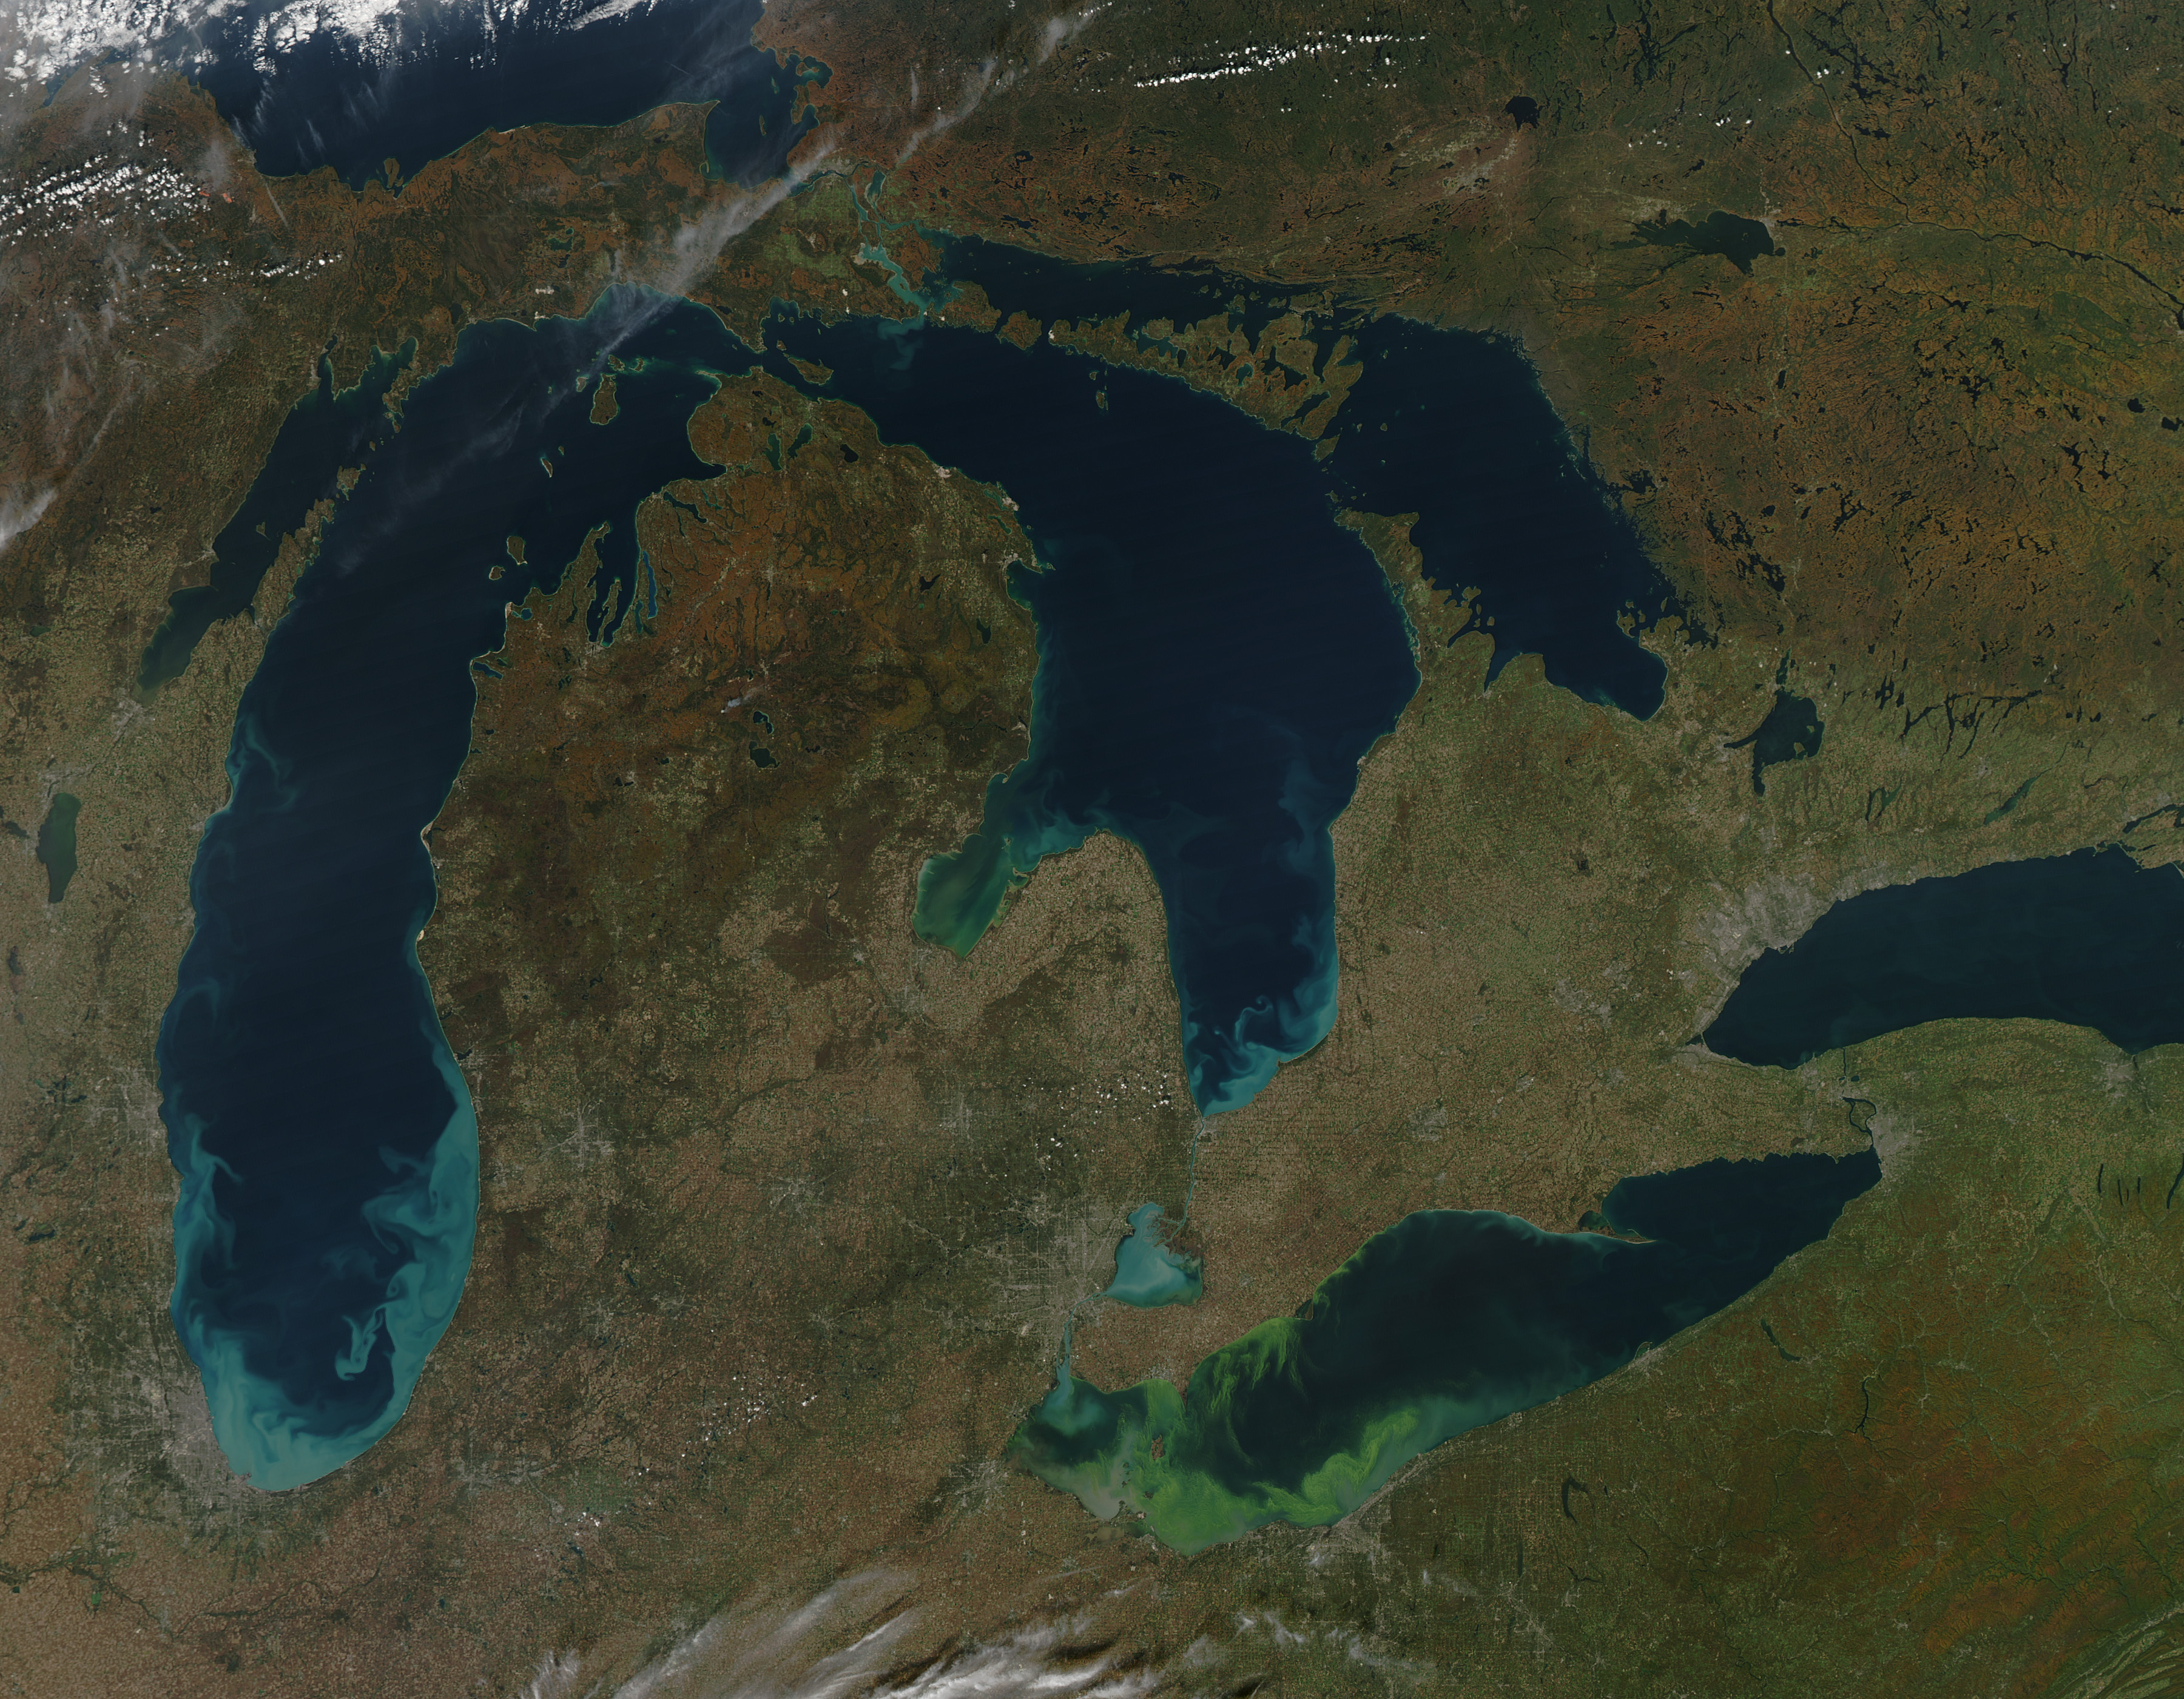
\includegraphics[scale = 0.15]{assets/algalbloom.jpg}
                        \caption{Great Lakes: October 9, 2011}
                  \end{wrapfigure}
                  

                \begin{itemize}
               		\item Drinking water is polluted.
					\item Local residents and visitors are prevented from boating, swimming, and visiting Lake Erie shorelines.
					\item Nearby residents are vulnerable to illnesses caused by the toxins. 
					\item Toxins can result in the death of marine life, and severely impact an aquatic ecosystem.
				\end{itemize}
                    \vspace*{3mm}
                \end{block}
                %%%%%%%%%%%%%%%%%%%%%%%%%%%%%%%%%%%
                %
                % Design
                %
                %%%%%%%%%%%%%%%%%%%%%%%%%%%%%%%%%%%
                \begin{exampleblock}{\textsc{\textbf{System Design}}}
					   \begin{figure}
                    		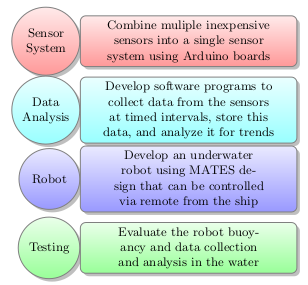
\includegraphics[scale = 4]{assets/diagram}
                    	\caption{Different portions comprising the system}
                    	\end{figure}
  				
  					\begin{block}{Sensor System Prototypes}
                    \begin{enumerate}
    	                \item 
                    	Extend sensors with 30ft cable, keep the board and power on surface.
						\item  Create a waterproofed unit to house sensors and boards on the robot.
						%\begin{itemize}		
						%	\item Waterproof casing.
						%	\item On-board battery.
						%	\item Micro-SD card.
						%\end{itemize}
					\end{enumerate}
					
                    % \begin{figure}
                    %     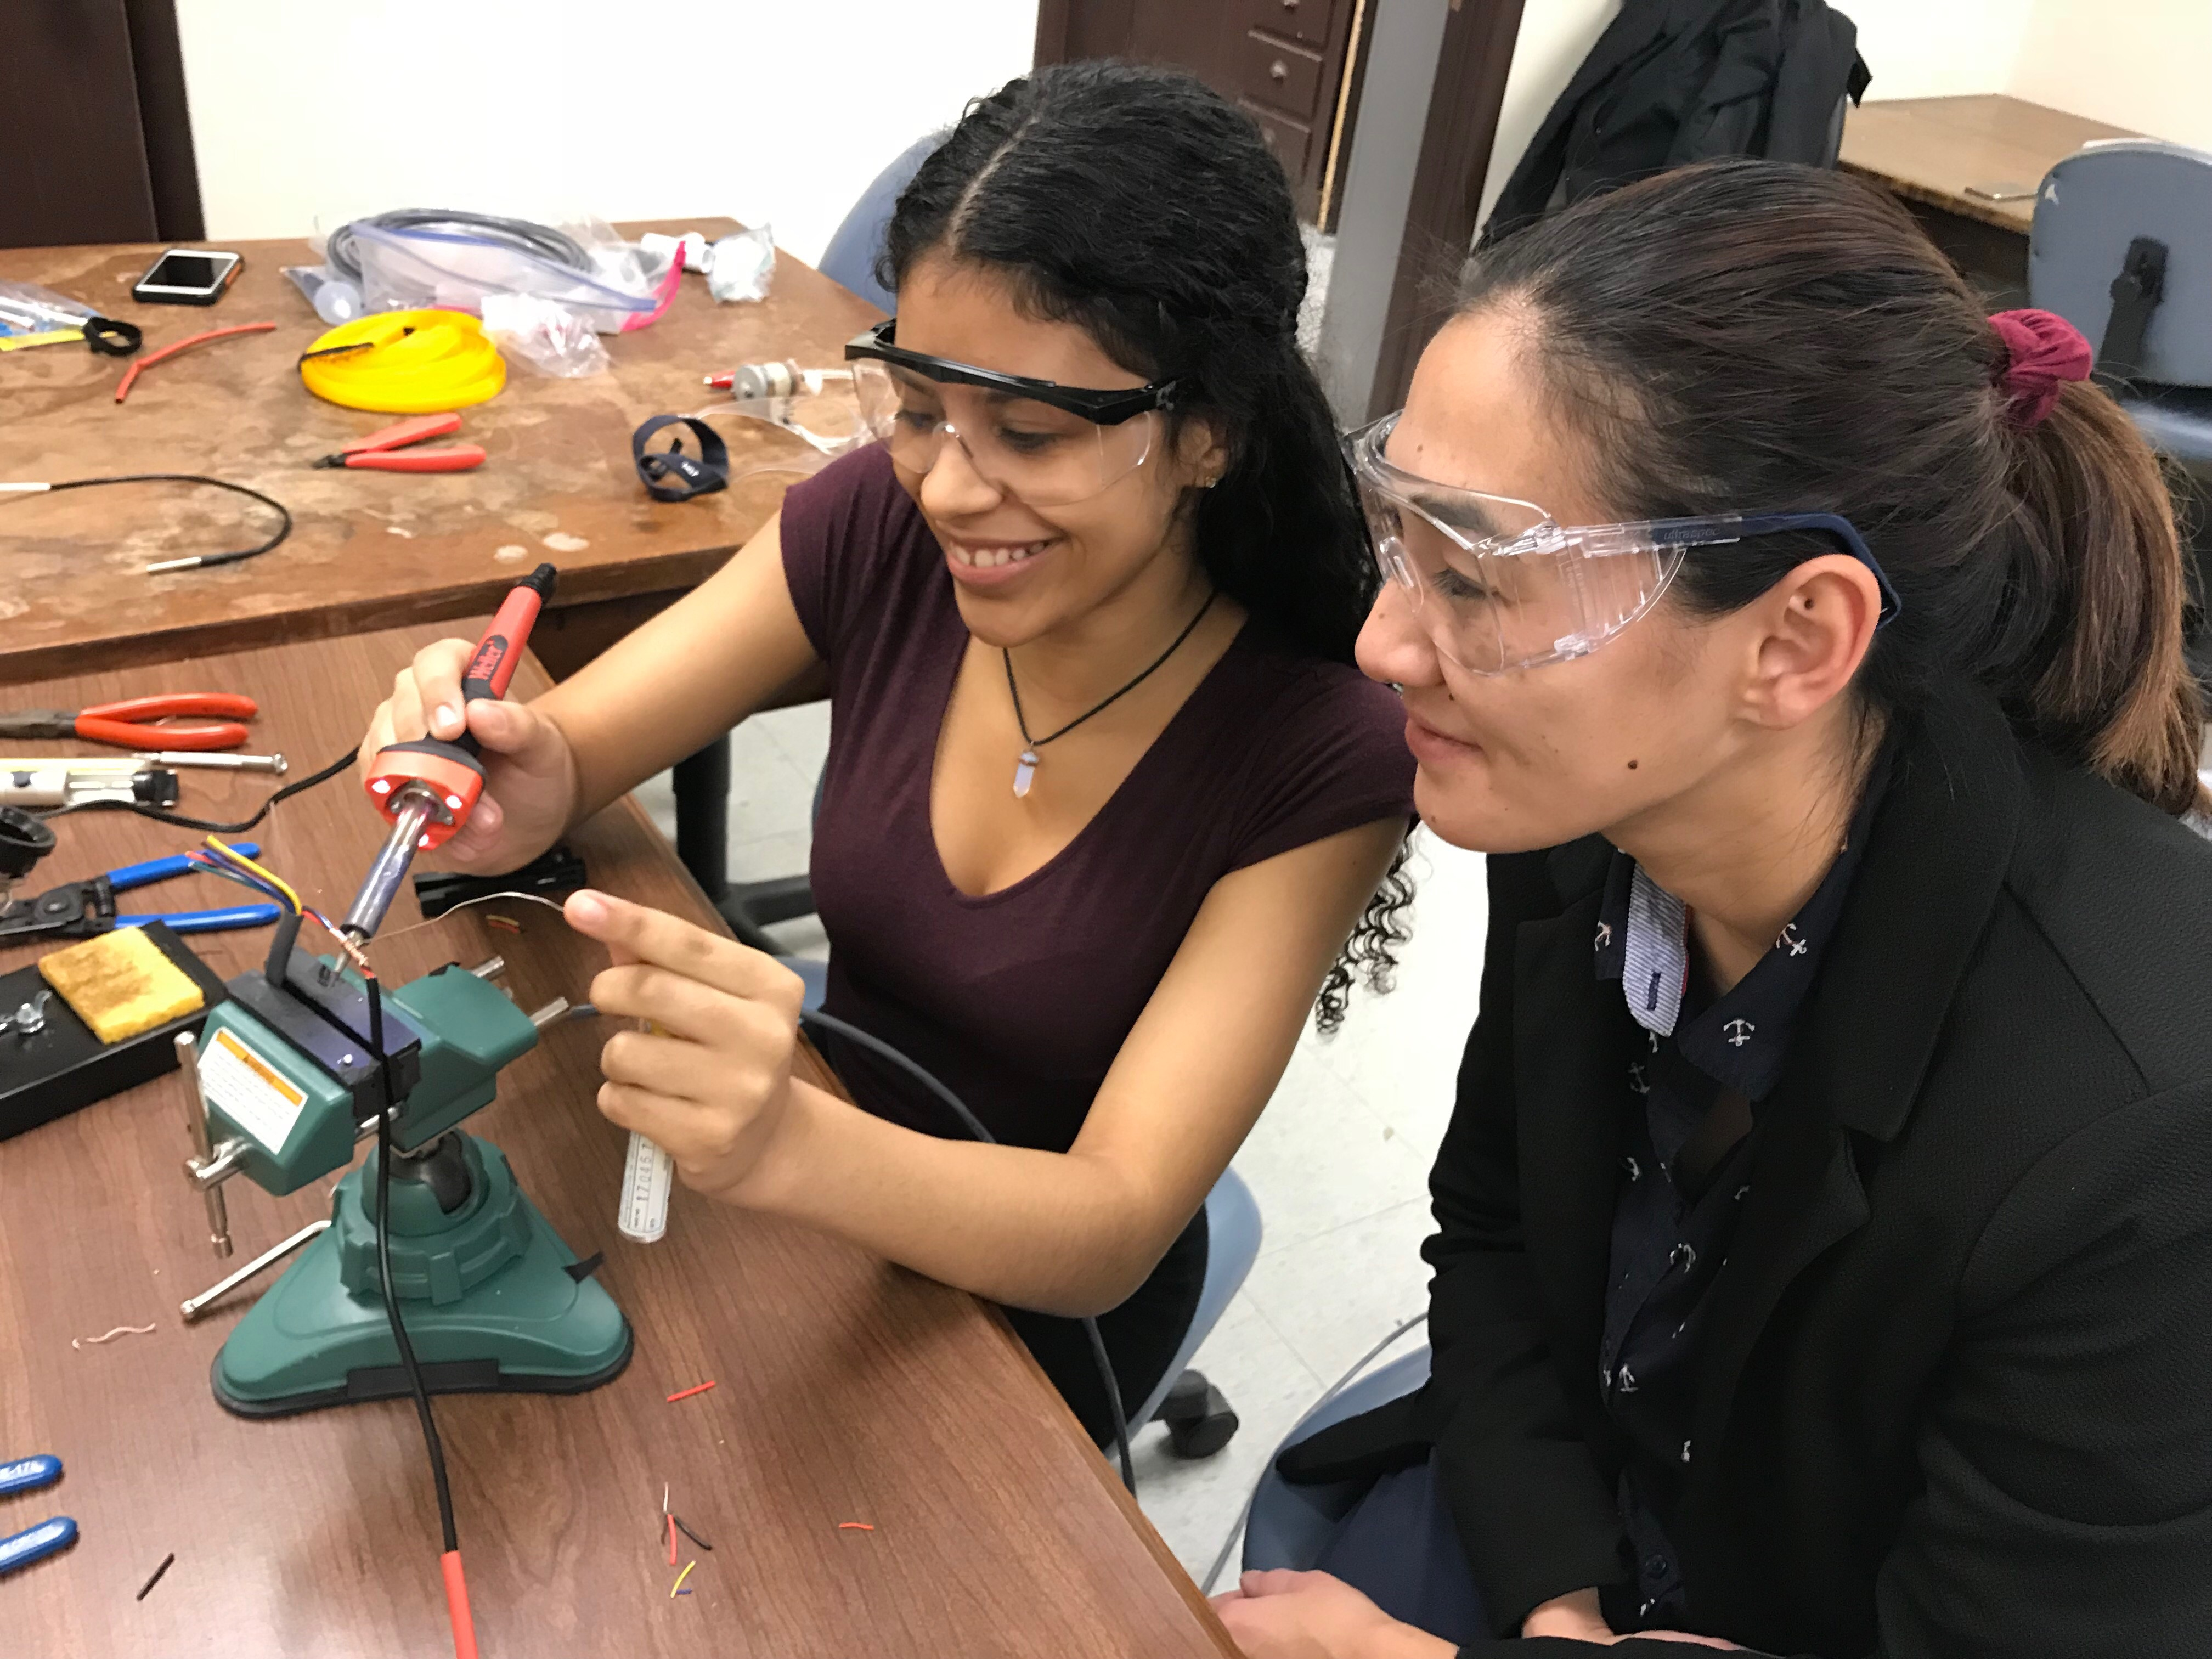
\includegraphics[scale = 0.15]{assets/IMG_9097.JPG}
                    %     \caption{Soldering wires}
                    % \end{figure}

                    \begin{center}
                    \begin{figure}
                    \begin{tabular}{cc}
                    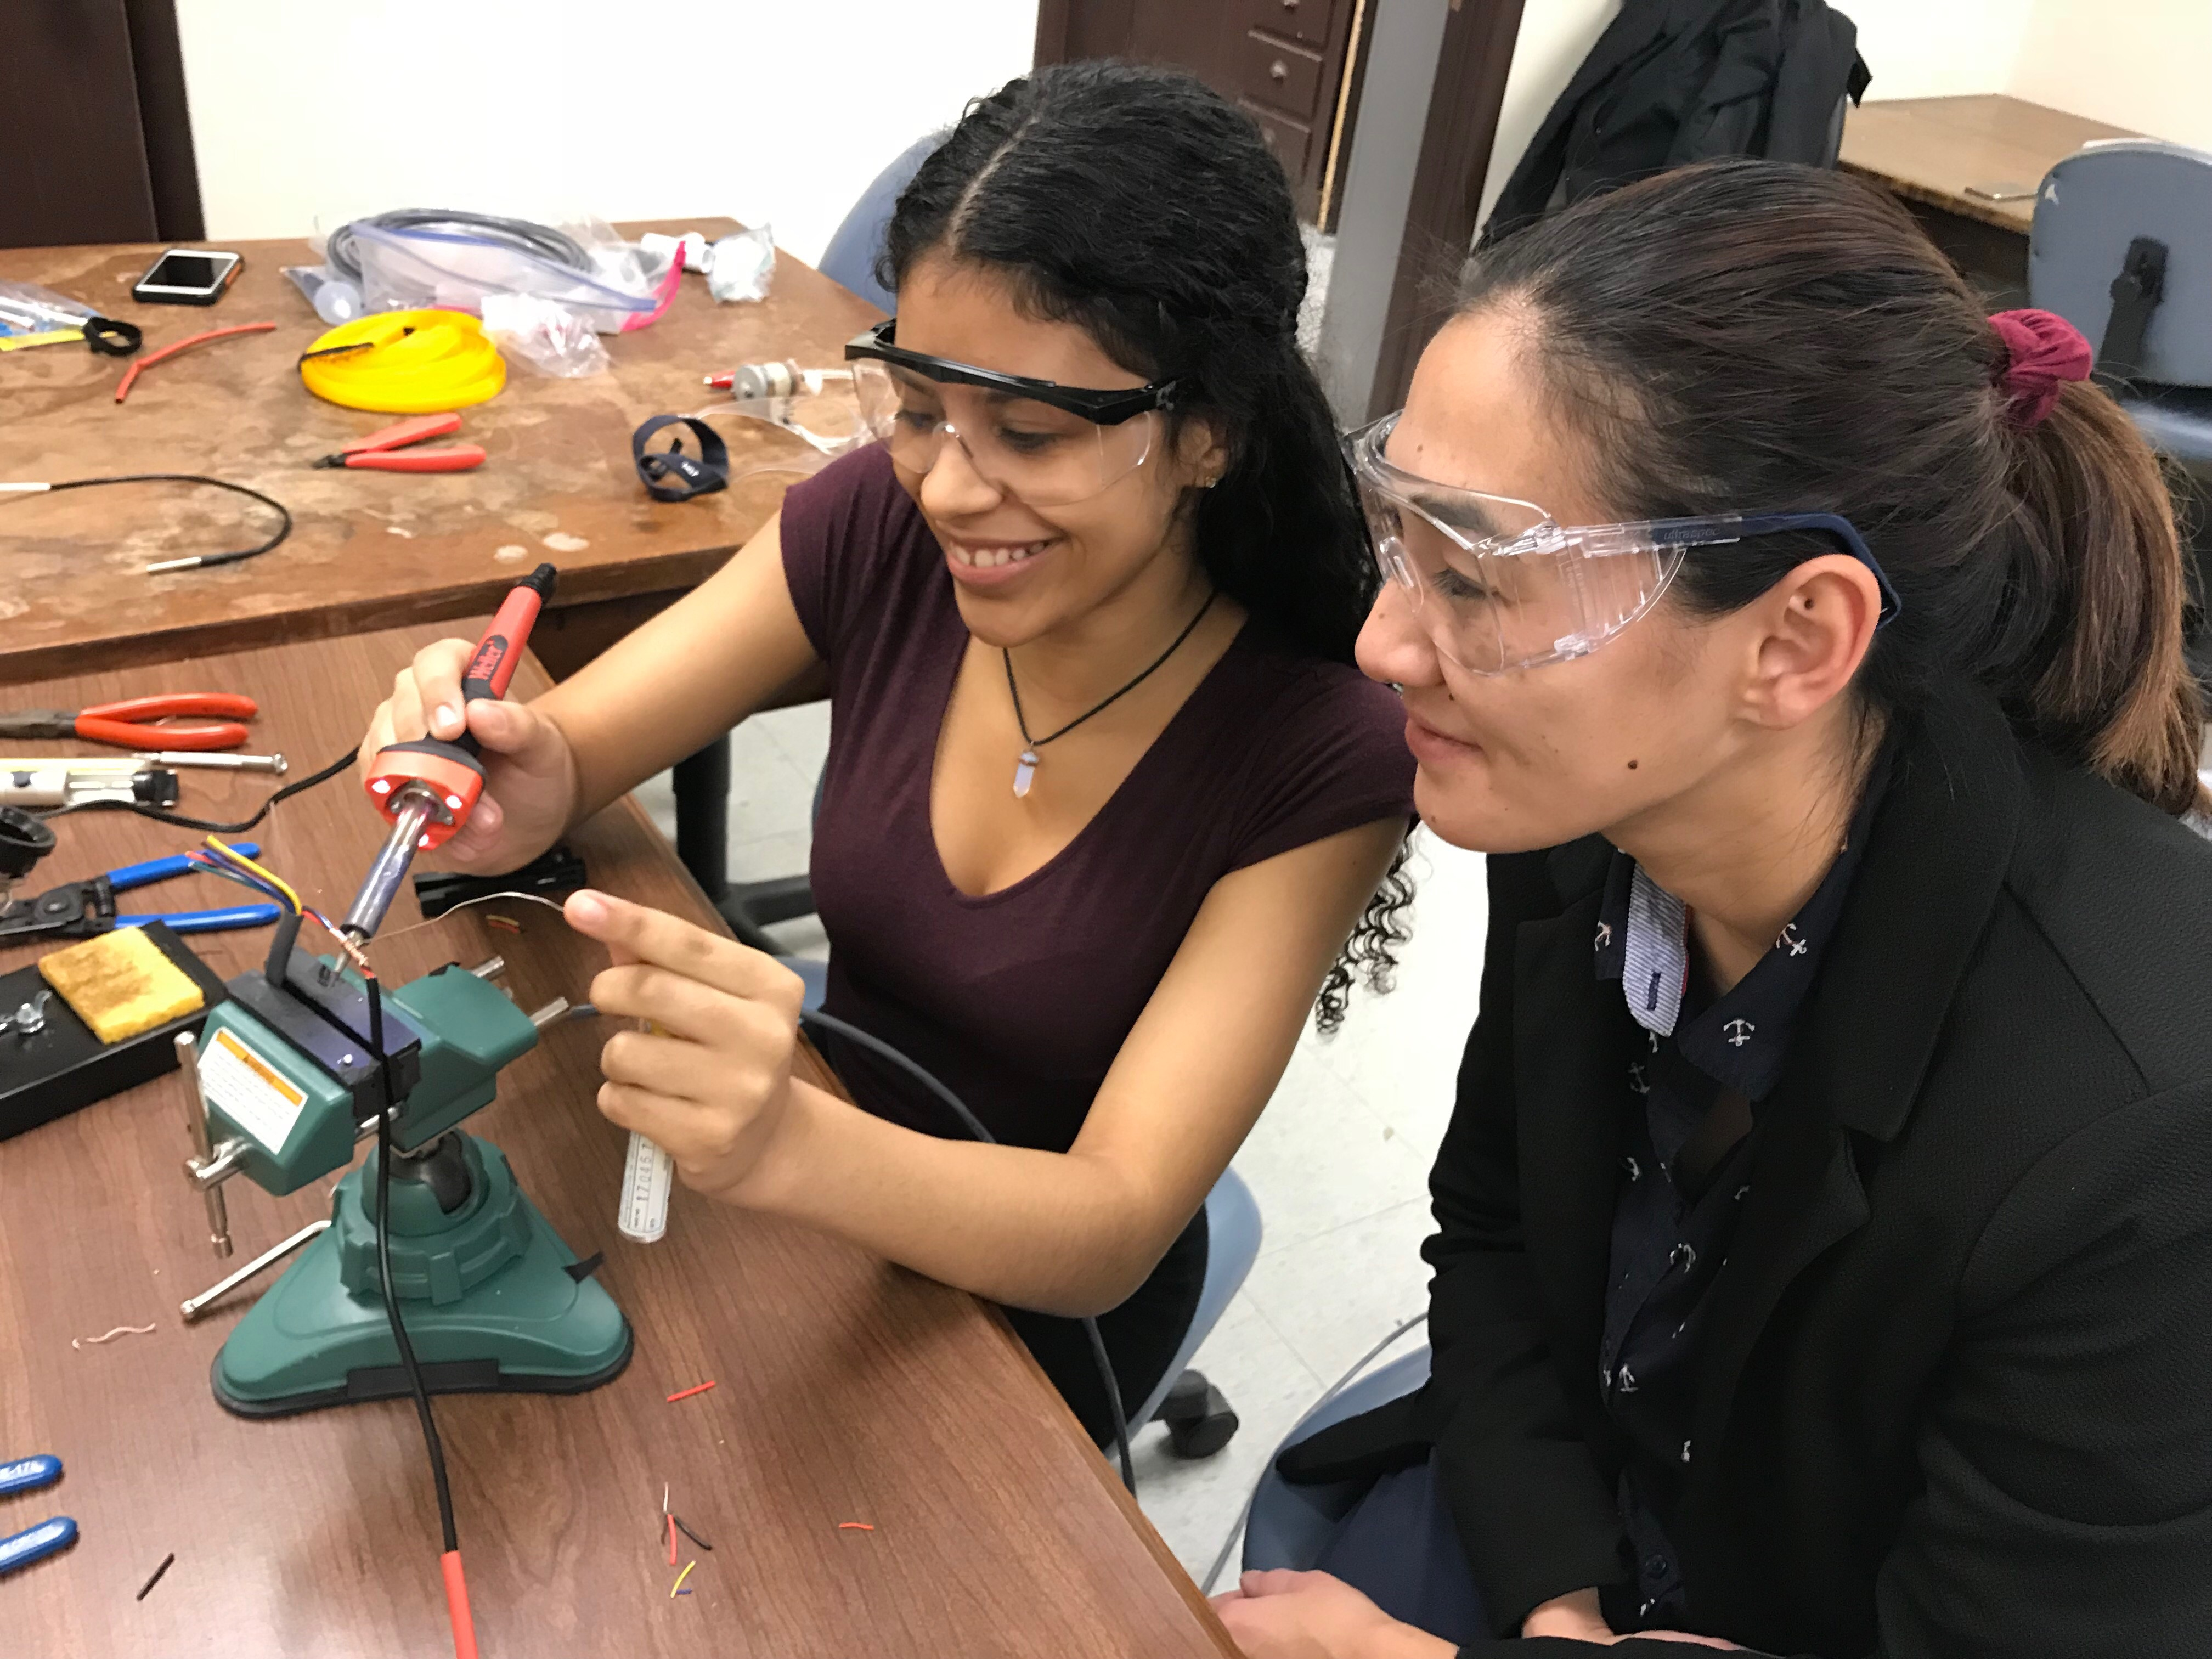
\includegraphics[scale = 0.15]{assets/IMG_9097.JPG}
                    \hspace*{5mm}
                    &
                    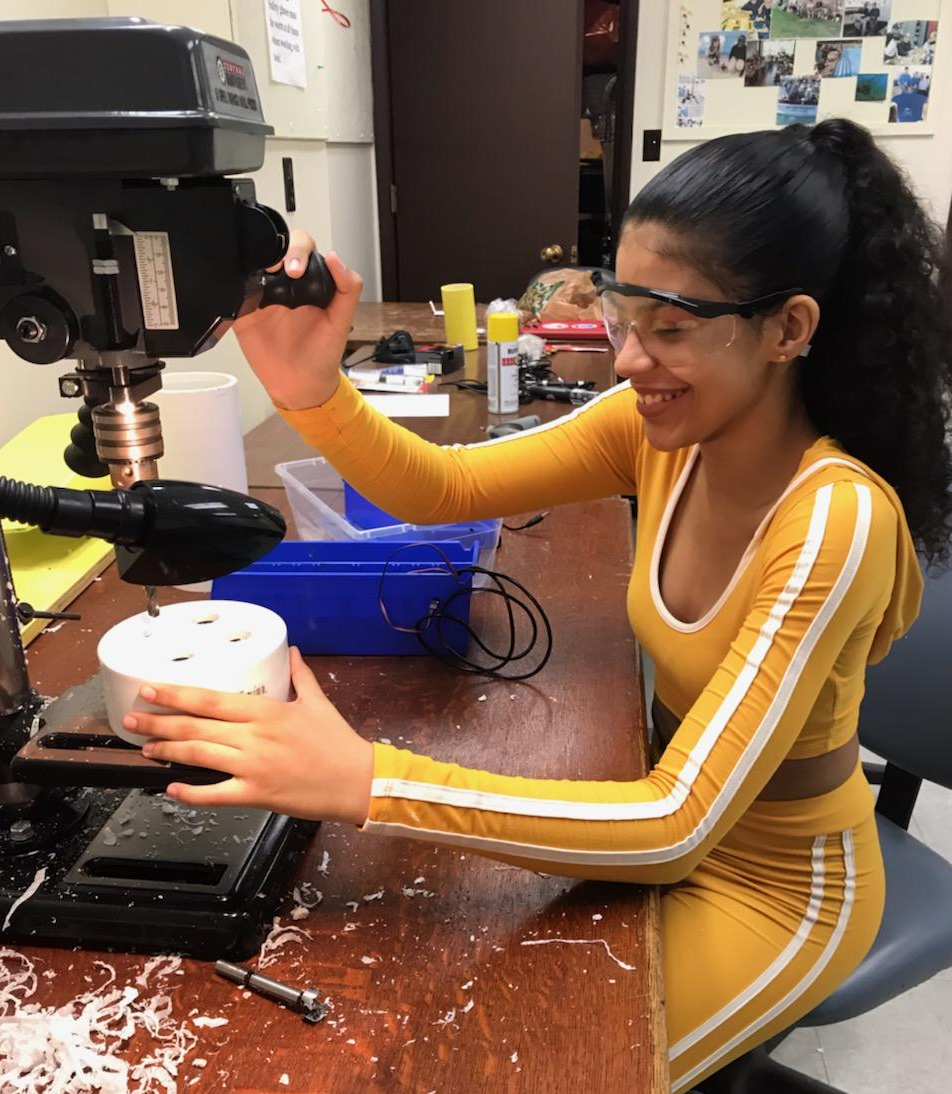
\includegraphics[scale = 0.42]{assets/meworking1}
                    \end{tabular}
                    \caption{Soldering sensor wires \hspace{30mm} Drilling holes for sensors}
                    \end{figure}
                    \end{center}
                    
  					\end{block}
                \end{exampleblock}
            \end{column}

            %%%%%%%%%%%%%%%%%%%%%%%%%%%%%%%%%%%%%%%%%%%%%%%%%%%%%%%%%%%%%%%%%%%%%
            %
            % Right column - Outcomes
            %
            %%%%%%%%%%%%%%%%%%%%%%%%%%%%%%%%%%%%%%%%%%%%%%%%%%%%%%%%%%%%%%%%%%%%%
            \begin{column}{.5\linewidth}

                %%%%%%%%%%%%%%%%%%%%%%%%%%%%%%%%%%%
                %
                % Robot
                %
                %%%%%%%%%%%%%%%%%%%%%%%%%%%%%%%%%%%
                \begin{block}{\textsc{Robotic Platform}}
                    \vspace*{3mm}
                    \begin{figure}
                    \centering
                        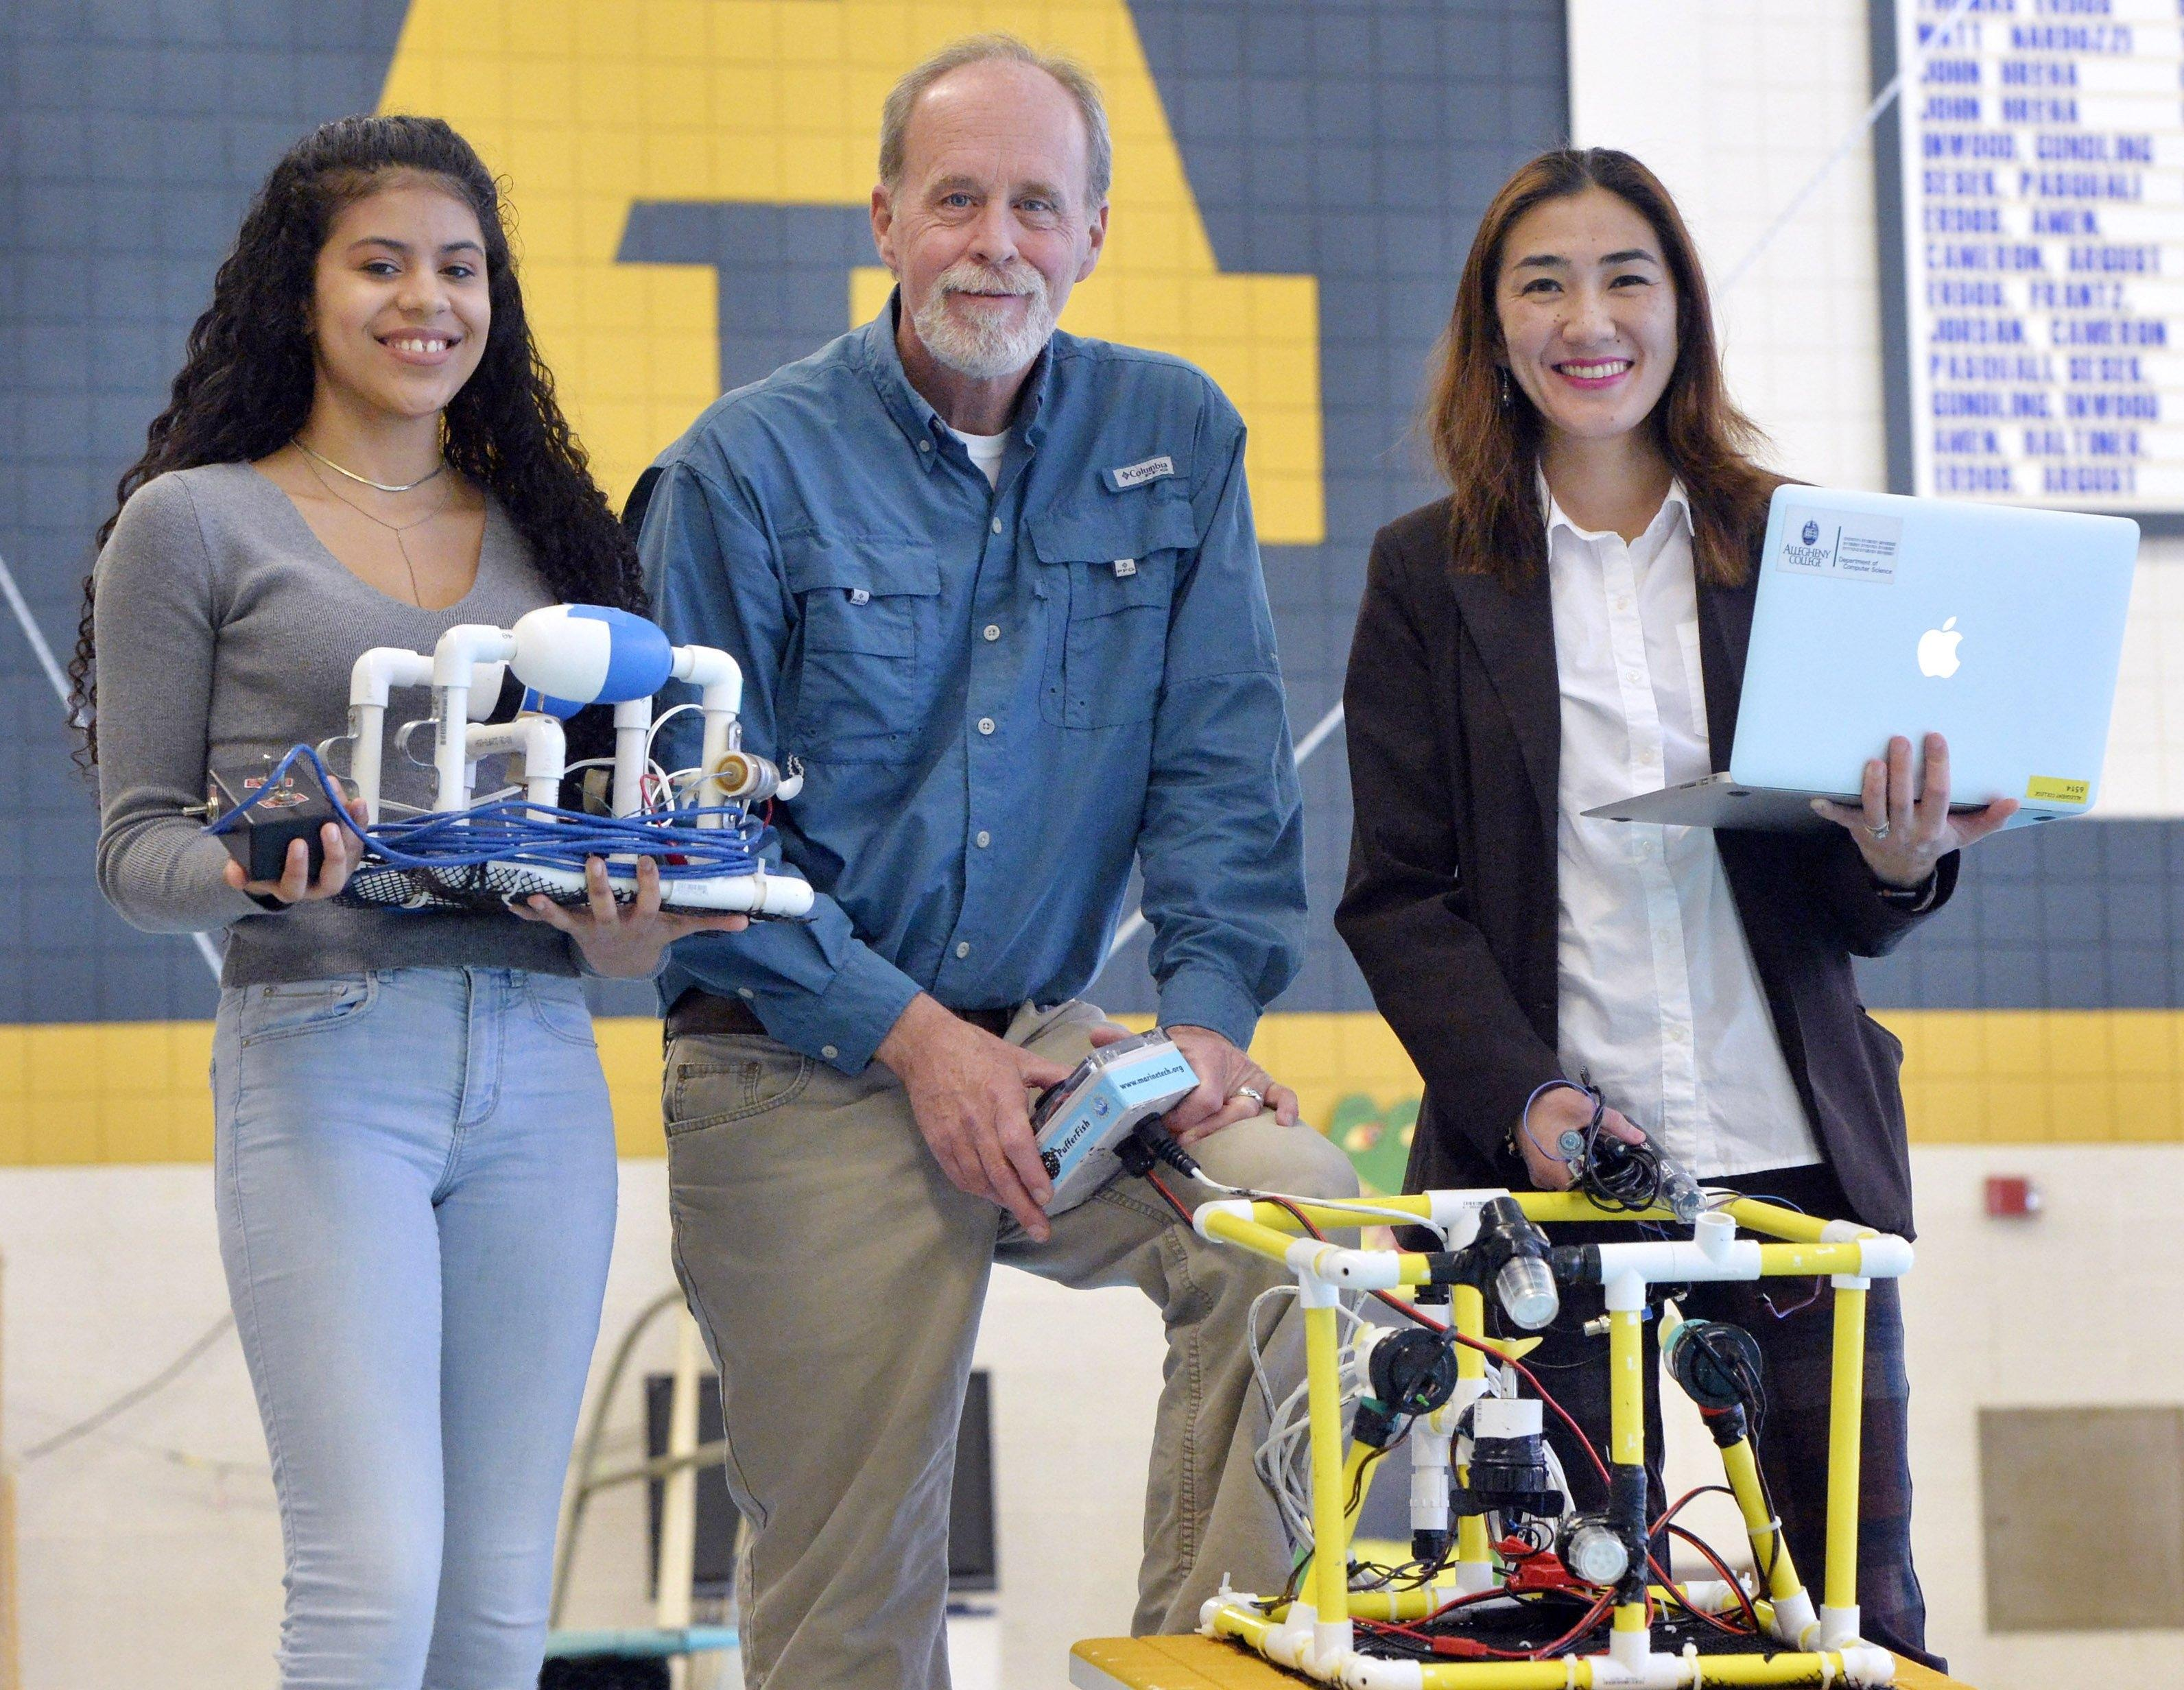
\includegraphics[scale = 0.9]{assets/group_pic.jpg}
                        \caption{Project Team with Different Robot Models}
                    \end{figure}
                    
                    \begin{itemize}
                    	\item Two remotely operated robotic models were used: the SeaPerch robot (left) and the MATE prototype (right). 
                    	\item Both robotic platforms are constructed with PVC pipe, mesh, propellers, solder, and other materials, and are easily deconstructable.
                    	\item This portion of the project was possible to the collaborative educational project between Allegheny College and Crawford Central School District, enabling middle school students to construct these units.
                    \end{itemize}
                    
                    \vspace*{3mm}
                \end{block}
                %%%%%%%%%%%%%%%%%%%%%%%%%%%%%%%%%%%
                %
                % Sensors
                %
                %%%%%%%%%%%%%%%%%%%%%%%%%%%%%%%%%%%
                \begin{block}{\textsc{Sensors}}
                    \vspace*{3mm}
                    
                    \begin{wrapfigure}{l}{0.45\textwidth}
                        \centering
                        \includegraphics[width=0.35\textwidth]{assets/sensors.jpg}
                        \caption{Arduino board and sensors}
                    \end{wrapfigure}
                    To complete our sensor system we used a collection of sensors, Arduino boards, and programs. 
                    \begin{itemize}
                    	\item pH, conductivity, temperature, dissolved oxygen sensors were used. 
                     
                    	\item These sensors are all connected to an Arduino board for automatic data collection and analysis. 
                     	\item Waterproofed sensors on this robotic system allows for data to be collected for several hours at a time, which is then transmitted to the analytics software.
                     \end{itemize}
                     
                    \vspace*{3mm}
                \end{block}

                %%%%%%%%%%%%%%%%%%%%%%%%%%%%%%%%%%%
                %
                % Results
                %
                %%%%%%%%%%%%%%%%%%%%%%%%%%%%%%%%%%%
                \begin{alertblock}{\textsc{Testing and Future Work}}
                    \vspace*{3mm}
                    \begin{itemize}
                    	\item First, software and the sensor data collection, management and analysis were evaluated.
                    	\item Then, completed robotic system was tested in the pool water.
                    	\item In May, measurements from Lake Erie will be taken at different levels of the water column. 
                    	\item The results of this project, including the collected data and its analysis, will be shared with other researchers and will be used to help students understand variations in water quality measurements. 
                    	%\item The data retrieved can be used to protect coastal environments and surrounding communities.
                    \end{itemize}

                    % \begin{figure}
                    %     \includegraphics[scale = 2.5]{}
                    %     \caption{}
                    % \end{figure}
                    
                    \vspace*{3mm}
                \end{alertblock}
            \end{column}


        \end{columns}
    \end{frame}
\end{document}
